\documentclass[12pt]{article}
\usepackage[a4paper, total={6in, 8in}]{geometry}
\usepackage{tikz}

\usetikzlibrary{automata,shapes.multipart}

\begin{document}
	\section*{Entwurfsskizze}

	Das Programm ist aufgeteilt in Frontend und Backend. Das Frontend ist verantwortlich für das GUI und Events (Mausklicks, Knopfdrücke, etc.),
	sowie für das graphische Darstellen der Daten aus dem Backend.
	Das Backend ist verantwortlich für das Parsing des Inputs sowie für die Vorbereitung der Daten für das Frontend.

	\subsection*{Backend}
	\begin{figure}[h!]
		\begin{center}
			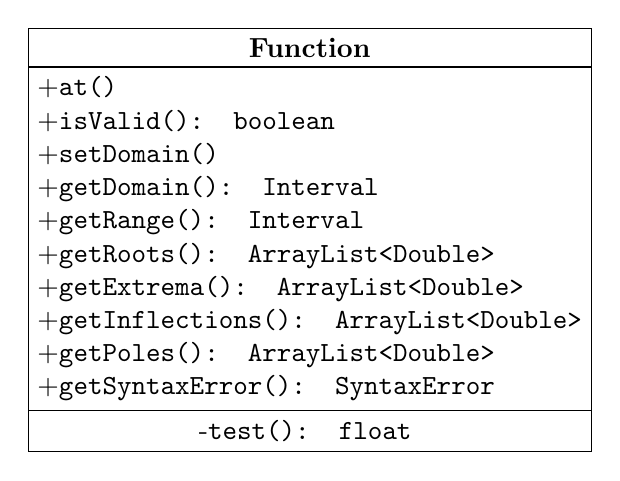
\begin{tikzpicture}[%
					every node/.style={%
						align=left,
						state,
						rectangle split,
						rectangle split parts=3
					}    
				]

				\node (function) at (0, 0) {%
					\textbf{Function}

					\nodepart{second}
					+\texttt{at()} \\
					+\texttt{isValid(): boolean} \\
					+\texttt{setDomain()} \\
					+\texttt{getDomain(): Interval} \\
					+\texttt{getRange(): Interval} \\
					+\texttt{getRoots(): ArrayList<Double>} \\
					+\texttt{getExtrema(): ArrayList<Double>} \\
					+\texttt{getInflections(): ArrayList<Double>} \\
					+\texttt{getPoles(): ArrayList<Double>}\\
					+\texttt{getSyntaxError(): SyntaxError}

					\nodepart{third}
					-\texttt{test(): float}
				};

				% \node (parser) [draw] at (0, -2) {Parser};
			\end{tikzpicture}
		\end{center}
		\caption{Test}
	\end{figure}

\end{document}